

\documentclass{report}
\setlength{\textwidth}{6.25in}
\setlength{\textheight}{8in}
\renewcommand{\baselinestretch}{1.3}
\oddsidemargin 20pt    %  Left margin on odd-numbered pages.
\evensidemargin 20pt   %  Note that \oddsidemargin = \evensidemargin
\topmargin 0pt
\usepackage{graphics}
\usepackage{graphicx}
\usepackage{epsfig}
\usepackage{url}



\begin{document}
\begin{titlepage}
	\begin{center}
%		{ \bf A}\\
%		\vspace{0.1in}
\large	{\bf Breast Cancer Detection using Machine Learning}\\
\vspace{0.1in}


		{ \bf Project Phase I Seminar Report\\
		{}	\vspace{0.1in} }
		\vspace{0.1in}
		
	
		{\it Submitted in the fulfillment of the requirement}\\
		{\it for the award of the degree of}\\
		\vspace{0.2in}
		{\bf Bachelor of Technology}\\
		\vspace{0.2in}
		{\bf in}\\
		\vspace{0.2in}
		{\bf INFORMATION TECHNOLOGY}\\
		\vspace{0.2in}
		{\it by}\\
		\vspace{0.1in}
		{\bf Chinmayee Bhoir(20160704)}\\
		{\bf Ashlesha Dule(20160712)}\\
		{\bf Neha Hakke(20160716)}\\
		{\bf Vibha Vaidya(20160761)}\\
		\vspace{0.3in}
			\vspace{0.1in}
				
		{\it Under the guidance of}\\
		\vspace{0.1in}
		{\large \textbf{Mr. Roshan Kotkondawar}}\\
		\vspace{0.1in}
		
		\begin{figure*}[h]
			\centerline{\psfig{figure=./batulogo.jpg,width=1in,height=1in}}
			\label{atcres}
		\end{figure*}
		
		{\small DEPARTMENT OF INFORMATION TECHNOLOGY \\
			{\large DR. BABASAHEB AMBEDKAR TECHNOLOGICAL UNIVERSITY}\\
			{\small Lonere-402103, Tal.-Mangaon, Dist.-Raigad (M.S.) INDIA.}\\
			2019-2020}
	\end{center}
\end{titlepage}


\pagenumbering{roman}

\newpage
\clearpage\thispagestyle{empty}


\begin{center}

\large{DR.BABASAHEB AMBEDKAR TECHNOLOGICAL UNIVERSITY}\\
\normalsize
Lonere,Raigad-Maharashtra,India-402103\\
\vspace{0.5in}


\begin{figure*}[h]
			\centerline{\psfig{figure=./batulogo.jpg,width=1in,height=1in}}
			\label{atcres}
		\end{figure*}
\vspace{0.5in}
\emph{\LARGE Certificate}\\[1.5cm]
\end{center}
\normalsize This is to certify that the Phase I on "Breast Cancer Detection using Machine Learning" is submitted by Ms. Chinmayee Bhoir(20160704), Ms. Ashlesha Dule(20160712), Ms. Neha Hakke(20160716), Ms. Vibha Vaidya(20160761) for the partial fulfilment of the requirements of the degree of Bachelor of Technology in Information Technology of the Dr.Babasaheb Ambedkar Technological University,Lonere is a bonafide work carried out during the academic year 2019-2020.\\[1.0cm]


\vfill
% Bottom of the page
\hspace{-0.2in}Mr. Roshan Kotkondawar\hspace{3.3in} Prof. S. M. Jadhav\\
(Project Guide)\hspace{3.85in} (Head of Department)\\
Information Technology\hspace{3.38in} Information Technology

\begin{flushleft}
Examiners:\\

1)..................(Prof. S.R.Sutar)\\


2)..................(Mr. Roshan Kotkondawar )\\[0.5cm]

Date:\\
Place:Lonere
\end{flushleft}









\chapter*{Acknowledgement\markboth{Acknowledgement}{Acknowledgement}}
It is our proud privilege and duty to acknowledge the kind of help and guidance received from several people in preparation of this report. It would not have been possible to prepare this report in this form without their valuable help, cooperation and guidance. First and foremost, we wish to record our sincere gratitude to \textbf{ Mr. Roshan Kotkondawar} for his constant support and encouragement in preparation of this report and for making available library and laboratory facilities needed to prepare this report. 

The presentation on \textbf{Breast Cancer Detection using Machine Learning} was very helpful to us in giving the necessary background information and inspiration in choosing this topic for the project. Their contributions and technical support in preparing this report are greatly acknowledged.

 Last but not the least, we wish to thank our parents for financing our studies in this college as well as for constantly encouraging us to learn engineering. Their personal sacrifice in providing this opportunity to learn engineering is acknowledged.  \\
\\
\\
\hspace*{4.5in} \textbf{Chinmayee Bhoir(20160704)}\\
\hspace*{4.5in} \textbf{Ashlesha Dule(20160712)}\\
\hspace*{4.5in} \textbf{Neha Hakke(20160716)}\\
\hspace*{4.5in} \textbf{Vibha Vaidya(20160761)}



\chapter*{Abstract\markboth{Abstract}{Abstract}}
Machine Learning is found useful in many areas and disease diagnosis is one such area. Many machine learning algorithms are available for prediction and diagnosis of breast cancer. Some of the machine learning algorithms are Naïve Bayes, Support Vector Machine (SVM), K-Nearest Neighbour (KNN) and Convolutional Neural Networks (CNN).The aim of this project is to compare and explain how Clustering and KNN algorithm provide better solution for diagnosing breast cancer. In this work, we will use K- Nearest neighbour algorithm for diagnosing breast cancer. We will implement K-Nearest Neighbour (KNN) algorithm for computing the final accuracy.



\newpage
\tableofcontents 
\newpage	
\pagenumbering{arabic}
\listoffigures
\newpage
\pagenumbering{arabic}

%

\chapter{Introduction}
\paragraph{}Breast cancer is cancer that develops from breast tissue. Signs of breast cancer may include a lump in the breast, a change in breast shape, dimpling of the skin, fluid coming from the nipple, a newly-inverted nipple, or a red or scaly patch of skin. In those with distant spread of the disease, there may be bone pain, swollen lymph nodes, shortness of breath, or yellow skin. 

\paragraph{}Risk factors for developing breast cancer include being female, obesity, lack of physical exercise, drinking alcohol, hormone replacement therapy during menopause, ionizing radiation, early age at first menstruation, having children late or not at all, older age, prior history of breast cancer, and family history. About 5–10\% of cases are due to genes inherited from a person's parents ,including BRCA1 and BRCA2 among others. Breast cancer most commonly develops in cells from the lining of milk ducts and the lobules that supply the ducts with milk. Cancers developing from the ducts are known as ductal carcinomas, while those developing from lobules are known as lobular carcinomas. In addition, there are more than 18 other sub-types of breast cancer. Some cancers, such as ductal carcinoma in situ, develop from pre-invasive lesions. The diagnosis of breast cancer is confirmed by taking a biopsy of the concerning lump. Once the diagnosis is made, further tests are done to determine if the cancer has spread beyond the breast and which treatments are most likely to be effective.


\paragraph{} The balance of benefits versus harms of breast cancer screening is controversial. A 2013 Cochrane review stated that it is unclear if mammographic screening does more good or harm. A 2009 review for the US Preventive Services Task Force found evidence of benefit in those 40 to 70 years of age, and the organization recommends screening every two years in women 50 to74 years of age. The medications tamoxifen or raloxifene may be used in an effort to prevent breast cancer in those who are at high risk of developing it. Surgical removal of both breasts is another preventative measure in some high risk women. In those who have been diagnosed with cancer, a number of treatments may be used, including surgery, radiation therapy, chemotherapy, hormonal therapy, and targeted therapy. Types of surgery vary from breast-conserving surgery to mastectomy. Breast reconstruction may take place at the time of surgery or at a later date. In those in whom the cancer has spread to other parts of the body, treatments are mostly aimed at improving quality of life and comfort. 

\paragraph{}Outcomes for breast cancer vary depending on the cancer type, the extent of disease, and the person's age. Survival rates in the developed world are high, with between 80 and 90\% of those in England and the United States alive for at least 5 years. In developing countries, survival rates are poorer. Worldwide, breast cancer is the leading type of cancer in women, accounting for 25\% of all cases. In 2018 it resulted in 2 million new cases and 627,000 deaths. It is more common in developed countries and is more than 100 times more common in women than in men. 
\begin{figure}[ht!]
\centering
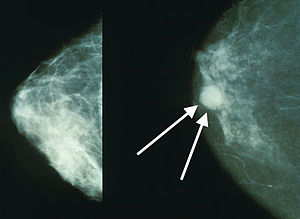
\includegraphics[width=100mm]{p1.jpg}
\caption{Mammograms showing a normal breast (left) and a breast with cancer (right, white arrows)\label{overflow}}
{\url{https://en.wikipedia.org/wiki/Breast_cancer#/media/File:Mammo_breast_cancer_wArrows.jpg}}
\end{figure}


\section{Sign and Symptoms:}
\begin{figure}[ht!]
\centering
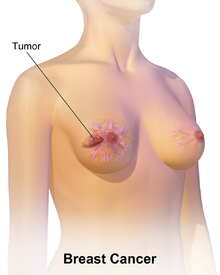
\includegraphics[width=60mm]{p2.png}
\caption{Tumours in Breast\label{overflow}}
{\url{https://en.wikipedia.org/wiki/Breast_cancer#/media/File:Breast_Cancer.png}}
\end{figure}

The first noticeable symptom of breast cancer is typically a lump that feels different from the rest of the breast tissue. More than 80\% of breast cancer cases are discovered when the woman feels a lump. The earliest breast cancers are detected by a mammogram. Lumps found in lymph nodes located in the armpits can also indicate breast cancer.

Indications of breast cancer other than a lump may include thickening different from the other breast tissue, one breast becoming larger or lower, a nipple changing position or shape or becoming inverted, skin puckering or dimpling, a rash on or around a nipple, discharge from nipple/s, constant pain in part of the breast or armpit and swelling beneath the armpit or around the collar bone. Pain is an unreliable tool in determining the presence or absence of breast cancer, but may be indicative of other breast health issues.

Another symptom complex of breast cancer is Paget's disease of the breast. This syndrome presents as skin changes resembling eczema; such as redness, discoloration or mild flaking of the nipple skin. As Paget's disease of the breast advances, symptoms may include tingling, itching, increased sensitivity, burning, and pain. There may also be discharge from the nipple. Approximately half the women diagnosed with Paget's disease of the breast also have a lump in the breast.

Inflammatory Breast Cancer presents with similar effects. Inflammatory Breast Cancer is a rare (only seen in less than 5\% of breast cancer diagnosis) yet aggressive form of breast cancer characterized by the swollen, red areas formed on the top of the Breast. The visual effects of Inflammatory Breast Cancer is a result of a blockage of lymph vessels by cancer cells. This type of breast cancer is seen in more commonly diagnosed in younger ages, obese women and African American women. As inflammatory breast cancer does not present as a lump there can sometimes be a delay in diagnosis.

In rare cases, what initially appears as a fibroadenoma (hard, movable non-cancerous lump) could in fact be a phyllodes tumor. Phyllodes tumors are formed within the stroma (connective tissue) of the breast and contain glandular as well as stromal tissue. Phyllodes tumors are not staged in the usual sense; they are classified on the basis of their appearance under the microscope as benign, borderline or malignant.

Malignant tumors can result in metastatic tumors— secondary tumors (originating from the primary tumor) that spread beyond the site of origination. The symptoms caused by metastatic breast cancer will depend on the location of metastasis. Common sites of metastasis include bone, liver, lung, and brain. When cancer has reached such an invasive state, it is categorized as a stage 4 cancer, cancers of this state are oftentimes fatal. Common symptoms of stage 4 cancer include unexplained weight loss, bone and joint pain, jaundice and neurological symptoms. These symptoms are called non-specific symptoms because they could be manifestations of many other illnesses.

Most symptoms of breast disorders, including most lumps, do not turn out to represent underlying breast cancer. Less than 20\% of lumps, for example, are cancerous, and benign breast diseases such as mastitis and fibroadenoma of the breast are more common causes of breast disorder symptoms.


\chapter{Machine Learning}
\section{What is Machine Learning?}
\paragraph{}Machine learning (ML) is the  scientific study of algorithms and statistical models that computer systems use to perform a specific task without using explicit instructions, relying on patterns and inference instead. It is seen as a subset of artificial intelligence. Machine learning algorithms build a mathematical model based on sample data, known as "training data", in order to make predictions or decisions without being explicitly programmed to perform the task. Machine learning algorithms are used in a wide variety of applications, such as email filtering and computer vision, where it is difficult or infeasible to develop a conventional algorithm for effectively performing the task.
\paragraph{}Machine learning is closely related to computational statistics, which focuses on making predictions using computers. The study of mathematical optimization delivers methods, theory and application domains to the field of machine learning. Data mining is a field of study within machine learning, and focuses on exploratory data analysis through unsupervised learning. In its application across business problems, machine learning is also referred to as predictive analytics

\section{What does it do? }

\paragraph{}It enables the computers or the machines to make data-driven decisions rather than being explicitly programmed for carrying out a certain task. These programs or algorithms are designed in a way that they learn and improve over time when are exposed to new data.

\section{Evolution of Machines}
\paragraph{}As you know, we are living in the world of humans and machines. The Humans have been evolving and learning from their past experience since millions of years. On the other hand, the era of machines and robots have just begun. You can consider it in a way that currently we are living in the primitive age of machines, while the future of machine is enormous and is beyond our scope of imagination.
\paragraph{}In today’s world, these machines or the robots have to be programmed before they start following your instructions. But what if the machine started learning on their own from their experience, work like us, feel like us, do things more accurately than us? These things sound fascinating, Right? Well, just remember this is just the beginning of the new. 

\paragraph{}As you know, we are living in the world of humans and machines. The Humans have been evolving and learning from their past experience since millions of years. On the other hand, the era of machines and robots have just begun. You can consider it in a way that currently we are living in the primitive age of machines, while the future of machine is enormous and is beyond our scope of imagination.

\section{Types of Machine Learning}
The types of machine learning algorithms differ in their approach, the type of data they input and output, and the type of task or problem that they are intended to solve.


\subsection{Supervised Learning}
Supervised learning algorithms build a mathematical model of a set of data that contains both the inputs and the desired outputs. The data is known as training data, and consists of a set of training examples. Each training example has one or more inputs and a desired output, also known as a supervisory signal. In the mathematical model, each training example is represented by an array or vector, sometimes called a feature vector, and the training data is represented by a matrix. Through iterative optimization of an objective function, supervised learning algorithms learn a function that can be used to predict the output associated with new inputs. An optimal function will allow the algorithm to correctly determine the output for inputs that were not a part of the training data. An algorithm that improves the accuracy of its outputs or predictions over time is said to have learned to perform that task. 

Supervised learning algorithms include classification and regression. Classification algorithms are used when the outputs are restricted to a limited set of values, and regression algorithms are used when the outputs may have any numerical value within a range. Similarity learning is an area of supervised machine learning closely related to regression and classification, but the goal is to learn from examples using a similarity function that measures how similar or related two objects are. It has applications in ranking, recommendation systems, visual identity tracking, face verification, and speaker verification.

In the case of semi-supervised learning algorithms, some of the training examples are missing training labels, but they can nevertheless be used to improve the quality of a model. In weakly supervised learning, the training labels are noisy, limited, or imprecise; however, these labels are often cheaper to obtain, resulting in larger effective training sets.

\subsection{Unsupervised Learning}
Unsupervised learning algorithms take a set of data that contains only inputs, and find structure in the data, like grouping or clustering of data points. The algorithms therefore learn from test data that has not been labelled , classified or categorized. Instead of responding to feedback, unsupervised learning algorithms identify commonalities in the data and react based on the presence or absence of such commonalities in each new piece of data. A central application of unsupervised learning is in the field of density estimation in statistics, though unsupervised learning encompasses other domains involving summarizing and explaining data features.

Cluster analysis is the assignment of a set of observations into subsets (called clusters) so that observations within the same cluster are similar according to one or more predesignated criteria, while observations drawn from different clusters are dissimilar. Different clustering techniques make different assumptions on the structure of the data, often defined by some similarity metric and evaluated, for example, by internal compactness, or the similarity between members of the same cluster, and separation, the difference between clusters. Other methods are based on estimated density and graph connectivity.

\subsection{Reinforcement Learning}
Reinforcement learning is an area of machine learning concerned with how software agents ought to take actions in an environment so as to maximize some notion of cumulative reward. Due to its generality, the field is studied in many other disciplines, such as game theory, control theory, operations research, information theory, simulation-based optimization, multi-agent systems, swarm intelligence, statistics and genetic algorithms. In machine learning, the environment is typically represented as a Markov Decision Process (MDP). Many reinforcement learning algorithms use dynamic programming techniques. Reinforcement learning algorithms do not assume knowledge of an exact mathematical model of the MDP, and are used when exact models are infeasible. Reinforcement learning algorithms are used in autonomous vehicles or in learning to play a game against a human opponent.

\chapter{Clustering}
\paragraph{}Clustering is the task of grouping a set of objects in such a way that objects in the same group (called a cluster) are more similar (in some sense) to each other than to those in other groups (clusters). It is a main task of exploratory data mining, and a common technique for statistical data analysis, used in many fields, including machine learning, pattern recognition, image analysis, information retrieval, bioinformatics, data compression, and computer graphics.

\paragraph{}Cluster analysis itself is not one specific algorithm, but the general task to be solved. It can be achieved by various algorithms that differ significantly in their understanding of what constitutes a cluster and how to efficiently find them. Popular notions of clusters include groups with small distances between cluster members, dense areas of the data space, intervals or particular statistical distributions. Clustering can therefore be formulated as a multi-objective optimization problem. The appropriate clustering algorithm and parameter settings (including parameters such as the distance function to use, a density threshold or the number of expected clusters) depend on the individual data set and intended use of the results. Cluster analysis as such is not an automatic task, but an iterative process of knowledge discovery or interactive multi-objective optimization that involves trial and failure. It is often necessary to modify data preprocessing and model parameters until the result achieves the desired properties.

\section{KNN  Algorithm}
The k-nearest neighbour algorithm (KNN) is a non-parametric method used for classification and regression. In both cases, the input consists of the k closest training examples in the feature space. The output depends on whether KNN is used for classification or regression:
\begin{itemize}
\item In KNN classification, the output is a class membership. An object is classified by a plurality vote of its neighbours, with the object being assigned to the class most common among its k nearest neighbours (k is a positive integer, typically small).If k = 1, then the object is simply assigned to the class of that single nearest neighbour.
\item In KNN regression, the output is the property value for the object. This value is the average of the values of k nearest neighbours
\end{itemize}


KNN is a type of instance-based learning, or lazy learning, where the function is only approximated locally and all computation is deferred until classification.
Both for classification and regression, a useful technique can be to assign weights to the contributions of the neighbors, so that the nearer neighbors contribute more to the average than the more distant ones. For example, a common weighting scheme consists in giving each neighbor a weight of 1/d, where d is the distance to the neighbor.
 
The neighbors are taken from a set of objects for which the class (for k-NN classification) or the object property value (for k-NN regression) is known. This can be thought of as the training set for the algorithm, though no explicit training step is required.
A peculiarity of the KNN algorithm is that it is sensitive to the local structure of the data.

\section{Algorithm}
The training examples are vectors in a multidimensional feature space, each with a class label. The training phase of the algorithm consists only of storing the feature vectors and class labels of the training samples.
In the classification phase, k is a user-defined constant, and an unlabeled vector (a query or test point) is classified by assigning the label which is most frequent among the k training samples nearest to that query point.

A commonly used distance metric for continuous variables is Euclidean distance. For discrete variables, such as for text classification, another metric can be used, such as the overlap metric (or Hamming distance). In the context of gene expression microarray data, for example, k-NN has been employed with correlation coefficients, such as Pearson and Spearman, as a metric. Often, the classification accuracy of k-NN can be improved significantly if the distance metric is learned with specialized algorithms such as Large Margin Nearest Neighbor or Neighbourhood components analysis.

A drawback of the basic "majority voting" classification occurs when the class distribution is skewed. That is, examples of a more frequent class tend to dominate the prediction of the new example, because they tend to be common among the k nearest neighbors due to their large number.[4] One way to overcome this problem is to weight the classification, taking into account the distance from the test point to each of its k nearest neighbors. The class (or value, in regression problems) of each of the k nearest points is multiplied by a weight proportional to the inverse of the distance from that point to the test point. Another way to overcome skew is by abstraction in data representation. For example, in a self-organizing map (SOM), each node is a representative (a center) of a cluster of similar points, regardless of their density in the original training data. KNN can then be applied to the SOM.

\subsection{Steps in KNN algorithm} 
\begin{enumerate}
\item Calculate “d(x, xi)” i =1, 2, . . . .., n; where d denotes the Euclidean distance between the points.
 
\item Arrange the calculated n Euclidean distances in non-decreasing order.  
\item Let k be a +ve integer, take the first k distances from this sorted list.  
\item Let k be a +ve integer, take the first k distances from this sorted list.  
\item Let ki denotes the number of points belonging to the ith class among k points  i.e. k 0 
\item If ki kj ij then put x in class i.
\end{enumerate}

\textbf {Example}

Classify whether a special paper tissue is good or not when x1=3 and x2=7  for k=3

\begin{center}
\begin{tabular}{ |c|c|c| } 
 \hline
 X1=Acid Durability & X2=Strength & Classification \\ 
\hline
7  & 7 & BAD \\ 
\hline
 7 & 4 & BAD\\ 
 \hline
3 & 4 & GOOD\\ 
 \hline
1 & 4 & GOOD \\ 
 \hline
\end{tabular}
\end{center}

$Euclidean Distance=\sqrt{(X1-x1)^2+(X2-x2)^2}$
\\

\begin{itemize}
\item $ E1=\sqrt{(7-3)^2+(7-7)^2}=4    \hspace*{0.3in}        rank=3   \hspace*{0.3in}           Bad $
\item $E2=\sqrt{(7-3)^2+(4-7)^2}=5         \hspace*{0.3in}            rank=4 $
\item  $E3=sqrt{(3-3)^2+(4-7)^2}=3             \hspace*{0.3in}        rank=1        \hspace*{0.3in}        Good    $
\item  $E4=\sqrt{(1-3)^2+(4-7)^2}=3.6        \hspace*{0.3in}           rank=2       \hspace*{0.3in}          Good$
\end{itemize}

\section{Advantages}
\begin{itemize}
\item The algorithm is simple and easy to implement.  
\item There’s no need to build a model, tune several parameters, or make additional assumptions.
\item The algorithm is versatile. It can be used for classification, regression, and search (as we will see in the next section).
\end{itemize}

\section{Disadvantages}
\begin{itemize}
\item The algorithm gets significantly slower as the number of examples and/or predictors/independent variables increase.
\end{itemize}


\chapter{Dataset}
A data set (or dataset) is a collection of data. In the case of tabular data, a data set corresponds to one or more database tables, where every column of a table represents a particular variable, and each row corresponds to a given record of the data set in question. The data set lists values for each of the variables, such as height and weight of an object, for each member of the data set. Each value is known as a datum. Data sets can also consist of a collection of documents or files.
\section{Training Dataset}
\paragraph{}A training dataset is a dataset of examples used for learning, that is to fit the parameters (e.g., weights) of, for example, a classifier.
Most approaches that search through training data for empirical relationships tend to over fit the data, meaning that they can identify and exploit apparent relationships in the training data that do not hold in general. 

\section{Validation Dataset}
\paragraph{} A validation dataset is a dataset of examples used to tune the hyper parameters (i.e. the architecture) of a classifier. It is sometimes also called the development set or the "dev set". In artificial neural networks, a hyper parameter is, for example, the number of hidden units. It, as well as the testing set (as mentioned above), should follow the same probability distribution as the training dataset.


In order to avoid over fitting, when any classification parameter needs to be adjusted, it is necessary to have a validation dataset in addition to the training and test datasets. For example, if the most suitable classifier for the problem is sought, the training dataset is used to train the candidate algorithms, the validation dataset is used to compare their performances and decide which one to take and, finally, the test dataset is used to obtain[the performance characteristics such as accuracy, sensitivity, specificity, F-measure, and so on. The validation dataset functions as a hybrid: it is training data used by testing, but neither as part of the low-level training nor as part of the final testing.


\section{Test Dataset}

A test dataset is a dataset that is independent of the training dataset, but that follows the same probability distribution as the training dataset. If a model fit to the training dataset also fits the test dataset well, minimal over fitting has taken place (see figure below). A better fitting of the training dataset as opposed to the test dataset usually points to over fitting.

\chapter{Conclusion}
  
\begin{itemize}
\item The main purpose of this system is to predict breast cancer disease by using machine learning approach. 
\item Many times, symptoms for breast cancer are not detected early and patient can have severe health risk. This system can help in detecting breast cancer in early stage. 
\item The proposed system for detecting breast cancer is based on changes in breasts for individual person.
\item This method will prevent people from major health risks.  
\end{itemize}



\newpage

\thispagestyle{plain}
\newpage{}
\addcontentsline{toc}{chapter}{References}
\LARGE \textbf{References}
\large{}\newline






\begin{itemize}
	\item National Academies of Sciences, Engineering, and Medicine; Health and Medicine Division; Board on Health Care Services; National Cancer Policy Forum; Nass SJ, Patlak M, Zevon E, editors.
	\item Russel, S. and Norvig , P. (2003). Artificial Intelligence: A Modern Approach. 2nd Edition. New York: Prentice-Hall.
This is an excellent text on Artificial Intelligence, with several introductory chapters on Machine Learning.

	\item Mucherino A., Papajorgji P.J., Pardalos P.M. (2009) k-Nearest Neighbour Classification. Springer Optimization and Its Applications, volume 34. Springer, New York, NY
	

\end{itemize}


\end{document}